\section{Materiales y Métodos}

\subsection{Metodología}
 
 El propósito de este trabajo es proponer una metodología de minería de datos para logs de ACS. Para esto utilizaremos el proceso de descubrimiento de conocimiento en bases de datos\cite{Fayyad1996}, por sus siglas en inglés \textbf{KDD} (Knowledge Discovery in Databases). Este proceso consta de varias etapas:
 
\begin{enumerate}
	\item Identificación de una problemática a estudiar.
	\item Desarrollo de conocimiento previo del dominio de la aplicación y los objetivos del usuario final.
	\item Creación de un set de datos, en dónde se llevarán a cabo las operaciones.
	\item Limpieza y pre-procesamiento de los datos, eliminación de ruido, estrategias para el manejo de datos faltantes y análisis de las secuencias de tiempo.
	\item Proyección de los datos, búsqueda de características útiles que sean representativas del objetivo del problema. Reducción de los datos, utilizando reducción de dimensionalidad o métodos de transformación para disminuir el número de variables o encontrar una representación invariante para los datos.
	\item Implementación del método de procesamiento de datos.
	\item Búsqueda de patrones utilizando el método escogido, utilizando una representación de interés para reglas de clasificación, regresión, \textit{clustering}.
	\item Interpretación de los datos minados, en caso de que los resultados no sean los esperados es posible volver a iterar cualquiera de los pasos anteriores.
\end{enumerate}


\begin{figure}[H]
\centering
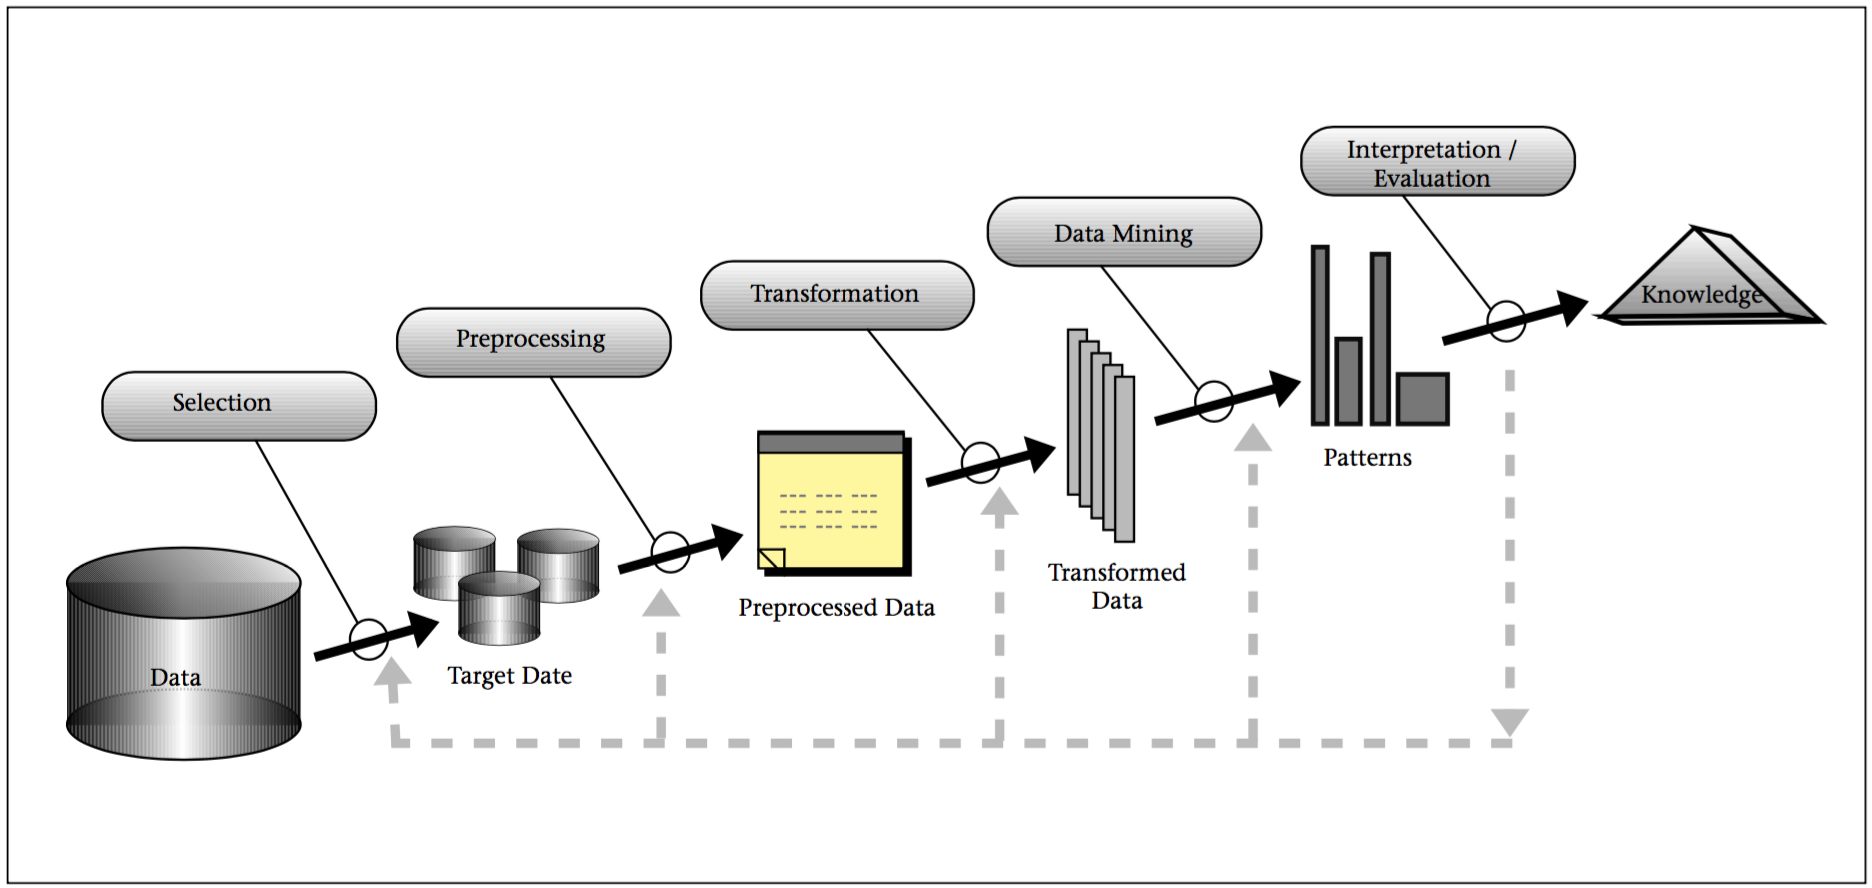
\includegraphics[scale=0.22]{img/kdd}
\caption{Proceso KDD}
\textbf{Fuente}: Fayyad \cite{Fayyad1996}
\end{figure}	


